\chapter{Estado da arte}
\pagestyle{simple} 

Esse capítulo tem por objetivo apresentar os principais conceitos abordados neste trabalho. Nas Seções \ref{areas-de-con} a \ref{biblios} são apresentados as áreas de conhecimento e ferramentas de software relacionadas a aplicabilidade de Inteligência Artificial e suas sub-áreas.

Nas últimas décadas vários trabalhos foram publicados nesse campo de pesquisa, demonstrando as mais diversas aplicações práticas dessas tecnologias. Na Seção \ref{trab-relacionados} estão dispostos esses trabalhos, de forma a demonstrar quais abordagens foram adotadas pelos autores para estudo das áreas em questão.

No âmbito da aplicação de IA para geração de sugestões em aplicações de \textit{e-commerce}, foco principal desse trabalho, o mercado mostra que essa é uma prática que veio para ficar. Isso ocorre pois essa tecnologia traz benefícios tanto para quem a aplica quanto para o usuário-alvo. Ao utilizá-la, os comerciantes desfrutam de um volume de vendas maior, visto que conseguem levar com mais assertividade seus produtos e serviços aos consumidores que estão interessados em adquirí-los. Os consumidores, da mesma forma, podem desfrutar de uma experiência mais agradável ao utilizar o \textit{e-commerce}, recebendo recomendações que lhe agradem e não apenas uma torrente de propagandas sem conexão com suas atividades cotidianas e hábitos de consumo.

Contudo, técnicas de IA trazem benefícios no dia a dia das pessoas em muitas outras áreas além do comércio, e frequentemente de maneira mais indireta. No campo das Ciências Sociais, por exemplo, já existem aplicações de IA na área do Direito, que permitem a advogados "trabalhar de forma mais eficiente e ampliar suas áreas de expertise" \citedirtp{alaire18} e na área financeira para "prever relatórios financeiros fraudulentos e crises financeiras" \citedirtp{clarence04}.

Há também algoritmos que se dedicam a análise de conteúdo textual, identificando casos de \textit{fake news} na Internet \cite{chitturi20} ou até atuando como "jornalistas robôs" capazes de "resumir artigos científicos e transformá-los em \textit{press releases} e matérias jornalísticas simples" \citedirtp{tatalovic18}.

No campo das Engenharias, IA já é utilizada no design otimizado de sistemas espaciais ligados por cabos \cite{chen19}, promover reuso de componentes de software e realizar análise de padrões de código \cite{wangoo18} e avaliar lances em licitações de construção civil \cite{sun11}.

Em relação às Ciências da Vida, na Medicina, a IA Watson desenvolvida pela empresa IBM foi utilizada com sucesso para "acelerar a identificação de novos candidatos a medicamentos e medicamentos-alvo através da exploração do potencial do \textit{Big Data}" \citedirtp{chen16}. Na agricultura de precisão, aplicações de identificação de imagem com IA foram utilizadas para "tratar aspectos relacionadas a detecção de doenças, qualidade do grão e fenotipagem" \citedirtp{patricio18}. 

Outro foco popular da área de IA é o desenvolvimento de \textit{chatbots}, agentes artificiais que podem atuar como interlocutores em uma conversação com um humano, auxiliar na aquisição de informações e oferecer respostas para perguntas \cite{wang18}. Eles podem ser aplicados em áreas tais como atendimento ao consumidor \cite{wessel20} e educação \cite{young19}.

\section{Conceitos e áreas de conhecimento} \label{areas-de-con}

\subsection {Inteligência Artificial}
Segundo \citedir{larousse99}, IA é um "conjunto de teorias e de técnicas empregadas com a finalidade de desenvolver máquinas capazes de simular a inteligência humana". 

De acordo com \citedirt{nikopoulos97}:

\begin{citacao}
A Inteligência Artificial é uma área de estudos da computação que se interessa pelo estudo e criação de sistemas que possam exibir um comportamento inteligente e realizar tarefas complexas com um nível de competência que é equivalente ou superior ao de um especialista humano.
\end{citacao}

Segundo John McCarthy, pioneiro que cunhou o termo Inteligência Artificial em 1955, o objetivo dessa área é "desenvolver máquinas que se comportam como se fossem inteligentes" \citedirt{wolf17}. Contudo, visto que não há consenso quanto ao que poderia ser considerado comportamento inteligente, essa definição é incompleta. A visão sobre o que é IA muda dependendo do momento histórico considerado, o que é descrito por \citeauthor{corduck04} (\citeyear{corduck04}, p.204, tradução nossa):

\begin{citacao}
É parte da história da área de Inteligência Artificial o fato de que toda vez que alguém descobre como fazer um computador fazer algo - jogar xadrez bem, resolver problemas simples mas relativamente informais - há um coro de críticos para dizer, ‘isso não é raciocínio’.
\end{citacao}

Dessa forma, algumas definições de IA preferem abordar a implementação da tecnologia do ponto de vista do desenvolvimento de \textit{software}. Conforme \citedirt{waterman85}:

\begin{citacao}
A Inteligência Artificial é uma sub-área da Ciência da Computação que objetiva desenvolver programas computacionais inteligentes. Esses programas são: solucionadores de problemas, programas que melhoram sua própria performance, programas que interpretam linguagens, programas que reconhecem esquemas visuais, enfim que se comportam de maneira que seria considerada inteligente se observada num ser humano.
\end{citacao}

De forma semelhante, segundo \citeauthor{pereira88} (\citeyear{pereira88}, p.2):

\begin{citacao}
A Inteligência Artificial é uma disciplina científica que utiliza as capacidades de processamento de símbolos da computação com o fim de encontrar métodos genéricos para automatizar actividades perceptivas, cognitivas e manipulativas, por via do computador.
\end{citacao}

Finalmente, de forma mais abrangente, \citedir{rich83} descreve IA como "o estudo de como fazer os computadores realizarem coisas que, no momento, as pessoas fazem melhor".

\subsection {Redes Neurais}
Segundo \citedirt{wolf17} redes neurais são "redes de células no cérebro de humanos e animais". Embora essa seja a definição literal do termo, quando o relacionamos com IA esse limita-se mais precisamente a descrever o processo de representação formal e reprodução artificial do funcionamento dos neurônios orgânicos. Como discorre o autor supracitado, "a partir do conhecimento do funcionamento de redes neurais naturais, tentamos modelá-las, simulá-las e até mesmo reconstruí-las em \textit{hardware}".

A replicação das redes neurais naturais de forma artificial se dá através do entendimento que o ser humano possui atualmente sobre o funcionamento de seu cérebro. Como descreve \citeauthor{rauber20} (\citeyear{rauber20}, p.3):

\begin{citacao}
(...) a pesquisa tenta entender o funcionamento da inteligência residente nos neurônios e mapeá-la para uma estrutura artificial, por exemplo uma combinação de \textit{hardware} e \textit{software}, assim transformando as redes neurais biológicas em redes neurais artificiais.
\end{citacao}

Similarmente, \citedirt{haykin01} define que:
\begin{citacao}
"Na sua forma mais geral uma rede neural é uma máquina que é projetada para modelar a maneira como o cérebro realiza uma tarefa particular ou função de interesse; a rede normalmente é implementada utilizando-se componentes eletrônicos ou é simulada por programação em um computador digital."
\end{citacao}

De forma mais pragmática, \citedir{osorio20} define que "as Redes Neurais Artificiais (RNAs) são ferramentas de Inteligência Artificial que possuem a capacidade de se adaptar e de aprender a realizar uma certa tarefa, ou comportamento, a partir de um conjunto de exemplos dados". 

\subsection {Machine Learning}
Segundo \citedir{azevedo19} "\textit{Machine learning} é um nome genérico dado a um conjunto de métodos para análise de dados desenvolvidos com o intuito de fazer previsão e classificação".

Segundo \citeauthor{mitchell97} (\citeyear{mitchell97}, tradução nossa) “\textit{Machine Learning} é uma sub-área da Inteligência Artificial diz respeito a questão de como construir programas de computador que melhoram automaticamente através da experiência”. Através de um processo de treinamento com diversas iterações um programa pode encontrar relações entre dados contidos em um modelo. 

Quantos aos principais tipos de algoritmos de \textit{Machine Learning}, \citedirt{stimpson14} descreve:

\begin{citacao}
"\textit{Machine learning} (ou \textit{data mining}) é uma ramificação da inteligência artificial que foca em algoritmos que identificam e aprendem as relações entre dados. Esses algoritmos geralmente são categorizados como não-supervisionados, que tentam identificar a estrutura intrínseca no dados, e supervisionados, que inferem uma função para relacionar dados a uma variável 'alvo'."
\end{citacao}

Quanto ao processo de inferência realizado por esses algoritmos, \citedirt{alpa20} descreve de forma sucinta:

\begin{citacao}
“De forma geral, nossa abordagem é começar com um modelo bem generalizado com muitos parâmetros, e esse modelo geral pode fazer todo tipo de tarefa dependendo de como seus parâmetros estão definidos. Aprender corresponde a ajustar os valores desses parâmetros de forma que o modelo coincida da melhor forma com os dados vistos durante o treinamento. Baseado nos dados de treinamento, o modelo generalizado, através de uma configuração particular de seus parâmetros, torna-se especializado na tarefa distinta que encontra-se entremeada aos dados. A versão do modelo que obtemos após o treinamento, a instanciação específica do modelo padrão, torna-se o algoritmo para a tarefa.“
\end{citacao}

\subsection {Deep Learning}
Segundo \citedirt{skansi18}, “considerando a visão mais simples possível, \textit{deep learning} é o nome de uma classe específica da redes neurais artificiais, que por sua vez são uma classe especial de algoritmos de \textit{Machine Learning}, aplicáveis a processamento de linguagem natural, \textit{computer vision} e robótica.”

Skansi também discorre sobre qual seria a maneira mais adequada de classificar o estudo de \textit{Deep Learning} em relação a outras áreas de conhecimento relacionadas:

\begin{citacao}
“Um número crescente de áreas da IA como raciocínio e planejamento, outrora bastiões da IA lógica (também chamada de \textit{Good Old-Fashioned AI}, ou GOFAI), estão sendo agora abordados de forma bem sucedida pelo \textit{deep learning}. Nesse sentido, pode-se dizer que \textit{deep learning} é uma abordagem de IA, e não apenas uma sub-área de uma sub-área da IA.”
\end{citacao}

De maneira mais formal e relacionada com o funcionamento de redes neurais, \citedirt{lecun15} descreve que um algoritmo de \textit{Deep Learning} “descobre estruturas intrincadas em grandes conjuntos de dados utilizando-se do algoritmo de \textit{backpropagation} para indicar como uma máquina deveria alterar seus parâmetros internos que são utilizados para computar a representação em cada camada a partir da representação na camada anterior.”

Segundo \citedirt{aggar18}:

\begin{citacao}
“A ideia base do \textit{deep learning} é de que a repetida composição de funções pode frequentemente reduzir os requerimentos no número de funções base (unidades computacionais) por um fator que é exponencialmente relacionado ao número de camadas da rede. Portanto, embora o número de camadas em uma rede aumente, o número de parâmetros requeridos para aproximar a mesma função reduz drasticamente. Isso aumenta o poder de generalização da rede. A ideia por trás da arquiteturas profundas é da que elas podem identificar melhor irregularidades repetidas em padrões de dados de forma a reduzir o número de unidades computacionais e portanto generalizar o aprendizado até mesmo em área do espaço amostral nos quais não existem exemplos.”
\end{citacao}

\section{Ambientes de desenvolvimento} \label{ambientes}
Existem vários ambientes de desenvolvimento para trabalhar com RNAs em diferentes linguagens. Para fins de contextualização, será realizada aqui uma breve comparação entre ambientes para a linguagem Python.

O Spyder é uma IDE de código aberto escrita em Python. Conforme o site oficial da ferramenta, ela oferece "uma combinação única de funcionalidades de edição avançada, análise, depuração e \textit{profiling} que podem ser encontradas em uma ferramenta de desenvolvimento completa com as capacidades de exploração de dados, execução interativa, inspeção profunda e visualização agradável de um pacote científico" \cite{spyder20}.

O Jupyter Notebook é uma IDE de código aberto para as linguagens Python, Julia e R desenvolvida pela Project Jupyter. Diferentes de outros ambientes do mesmo tipo, o Jupyter é uma aplicação \textit{web} que roda localmente e que possui um \textit{front-end} acessível pelo usuário através do navegador. Através da ferramenta é possível criar e compartilhar documentos que possuem código executável, equações, visualizações e textos explicativos. Além de \textit{Machine Learning}, a ferramenta pode ser utilizada também para simulação numérica, limpeza, transformação e visualização de dados \cite{jupyter20}.

O PyCharm é uma IDE de código fechado desenvolvida pela empresa JetBrains. O ambiente fornece várias funcionalidades focadas em tornar o processo de desenvolvimento mais ágil e aumentar produtividade, tais como completamento de código automático, checagem de erros em tempo real e recomendações de código baseadas no PEP8, manual de boas-práticas do Python. O PyCharm possui duas versões: a \textit{Community}, que é gratuita mas tem funcionalidades limitadas, e a \textit{Professional}, que não possui limitações mas é paga \cite{pycharm20}. 

O Visual Studio Code, uma IDE de código aberto desenvolvida pela Microsoft, é atualmente um dos ambientes de desenvolvimento mais amplamente utilizados no mundo \cite{so20}. Oferece suporte a uma grande variedade de linguagens, incluindo Python, bem como integração com ferramentas de depuração, versionamento e extensões produzidas pela mantenedora do software ou colaboradores \cite{microsoft20}.

\section{Bibliotecas} \label{biblios}
É possível construir e treinar redes neurais em qualquer linguagem de programação sem necessidade de instalação de bibliotecas ou \textit{frameworks}. Contudo, nesse caso é necessário escrever a implementação de algoritmo para inicializar pesos e \textit{biases}, funções de ativação, custo e \textit{backpropagation} com base em suas definições matemáticas formais \cite{peixeiro19}, o que torna o desenvolvimento de uma aplicação completa mais lento e trabalhoso, exigindo profundo conhecimento teórico de IA por parte do programador. 

Entretanto, principalmente no âmbito do desenvolvimento de \textit{software} comercial, agilidade e facilidade de uso e manutenção são pontos fundamentais. Portanto é comum que pesquisadores e programadores busquem ferramentas que tornem o processo mais acessível tanto para iniciantes quanto profissionais experientes na área. Para fins de contextualização, será realizada aqui uma breve comparação entre bibliotecas e \textit{frameworks} de IA e ML para a linguagem Python.

O Keras é uma biblioteca de código aberto para criação de redes neurais escrita em Python. Ela atua como uma API, uma interface consistente que permite ao usuário utilizar funções de mais baixo-nível descritas em bibliotecas matemáticas como TensorFlow e Theano \cite{brownlee19}. 

Segundo o site oficial, a biblioteca oferece "APIs simples e consistentes, minimiza o número de ações de usuário necessárias para casos de uso comuns e provém \textit{feedback} claro e prático em caso de erros por parte do usuário" \citedirtp{keras203}. O Keras se integra também com outros recursos e ferramentas, incluindo as do ecossistema TensorFlow.

O TensorFlow é uma biblioteca de código aberto que suporta linguagens como Python, JavaScript e Swift. Segundo a documentação oficial, a biblioteca possui "um completo e flexível ecossistema de ferramentas e recursos de comunidade que permitem que pesquisadores avancem o estado da arte do ML e que desenvolvedores construam e implantem facilmente aplicações com funcionalidades de ML" \citedirtp{tf20}. 

Esse ecossistema engloba ferramentas como o TensorFlow Cloud, que permite configurar o treinamento de RNAs em servidores na nuvem, e o TensorFlow Extended (TFX), pipeline para implantação de aplicações de \textit{Machine Learning}.

O Theano é uma biblioteca matemática escrita em Python. Segundo a documentação oficial, a biblioteca "permite que você defina, otimize e avalie expressões matemáticas envolvendo vetores multi-dimensionais de forma eficiente" \citedirtp{theano20}. Essas funcionalidades são utilizadas por outras bibliotecas como o Keras, que criam abstrações para tornar mais simples a construção de redes neurais mas que para atingir esse objetivo precisam de bibliotecas de apoio \cite{theano16}.

O PyTorch é uma biblioteca escrita em Python baseada na biblioteca Torch, originalmente escrita em Lua. A biblioteca provém funções para definição de funções matemáticas e computação de seus respectivos gradientes, bem como funcionalidades para processamento tanto em CPU quanto em GPU \cite{ketkar17}. 

O XGBoost é uma biblioteca que permite a implementação de algoritmos de \textit{Machine Learning} através de um \textit{framework} de \textit{Gradient Boosting}, que consiste "em um procedimento de aprendizado que consecutivamente ajusta novos modelos para prover uma estimativa mais precisa da variável de resposta" \citedirtp{natekin13}. Segundo pesquisa conduzida pela equipe do Keras, a XGBoost é a terceira ferramenta de ML mais utilizada por equipes que ficaram no top 5 das competições do site Kaggle em 2019 \cite{keras202}.

O LightGBM é um \textit{framework} de \textit{gradient boosting} escrito em Python mas com suporte para as linguagens C e R. Suporta também processamento em CPU e GPU \cite{lgbm20}. Segundo pesquisa conduzida pela equipe do Keras, a XGBoost é a segunda ferramenta de ML mais utilizada por equipes que ficaram no top 5 das competições do site Kaggle em 2019 \cite{keras202}.

\section{Sistemas de recomendação} \label{sist-rec} 
Visto que o objetivo principal do trabalho é criar um sistema de recomendação, essa seção irá descrever 3 abordagens populares para criação desse tipo de sistema: filtragem baseada em conteúdo, filtragem colaborativa e sistemas híbridos \cite{fressato19}. Outros métodos tem sido historicamente utilizados para a criação de sistemas de recomendação, tais como redes Bayesianas, clusterização \cite{li05} e a técnica denominada \textit{Horting}, baseada na teoria dos grafos \cite{aggarwal99}.

\subsection{Baseado em conteúdo}
Sistema que "recomenda itens com base em seus atributos" \cite{fressato19}. Um algoritmo que implementa essa abordagem correlaciona somente as características dos produtos comprados por um cliente, e como resultado recomendará outros produtos com características semelhantes. Como explica \citedirt{aciar07}:

\begin{citacao}
(...) Métodos baseados em conteúdo fazem recomendações através da análise da descrição dos itens que foram avaliados pelo usuário. Uma variedade de algoritmos tem sido proposta para analisar o conteúdo de documentos, e encontrar padrões nesse conteúdo pode servir como base para recomendações.
\end{citacao}

As características desejadas são inferidas pelo sistema com base nas interações entre cada usuário e os produtos no catálogo da plataforma de \textit{e-commerce}, como exemplifica \citedirt{burke02}:

\begin{citacao}
Outro paradigma de recomendação relevantes além de bases de conhecimento e recomendação colaborativa é o de recomendação baseada em conteúdo, na qual o sistema aprende um classificador para cada usuário baseado nas características de produtos curtidos e não curtidos.
\end{citacao}

Sistemas de recomendação baseados em conteúdo possuem fatores que limitam a quantidade e qualidade de suas sugestões, tais como:

\begin{itemize}
    \item A análise dos produtos pode acabar sendo rasa, especialmente quando não há muita informação sobre os itens ou essa informação está em formatos não-textuais (ex.: filmes, música, locais geográficos)  \cite{balabanovi97}
    \item A análise pode não ser satisfatória quando a descrição do produto é de difícil análise pelo computador, por exemplo, textos que envolvem opinião pessoal e discussão de ideias \cite{melville02}.
    \item Mesmo no caso de produtos que possuem descrição textual, essa nem sempre abrange todos os aspectos do produto. \cite{balabanovi97}
\end{itemize}

\subsection{Filtragem colaborativa}
Um algoritmo de filtragem colaborativa "recomenda itens de acordo com o comportamento de usuários similares" \cite{fressato19}. O que define essa similaridade depende do contexto que estamos analisando. Se os usuários são pessoas físicas, características como faixa etária, gênero e localização geográfica podem ser levadas em consideração. No caso de pessoas jurídicas, segmento de atuação e tamanho podem ser analisados.

De forma similar, \citedirt{chen18} define que a abordagem "faz recomendações para o usuário atualmente ativo utilizando vários históricos de avaliação de outros usuários sem analizar o conteúdo do recurso informacional". Quando cita "recurso informacional" o autor se refere ao produto, pois essa abordagem permite inferir sugestões sem que seja necessário conhecer dados do produto. 

\citedirt{kim01} faz um paralelo com a abordagem baseada em conteúdo:

\begin{citacao}
Um sistema de recomendação baseado em conteúdo sugere produtos para consumidores analisando o conteúdo dos itens pelos quais eles se interessaram no passado. (...) Em contraste, a técnica de filtragem colaborativa recomenda itens pelos quais consumidores similares se interessaram. 
\end{citacao}

Embora popularmente utilizados em aplicações de e-commerce, sistemas de FC frequentemente sofrem dos seguintes problemas:
\begin{itemize}
    \item Cold start (partida fria): o sistema é incapaz de gerar recomendações precisas para novos usuários do sistema, visto que esses não possuem um histórico de avaliação ou compra de produtos \cite{fressato19}
    \item Escalabilidade: o processamento de milhares ou milhões de produtos/clientes em um banco de dados de e-commerce demanda poder computacional e tempo \cite{lee04}
    \item Dispersão: visto que um e-commerce pode conter milhões de produtos, alguns desses itens serão pouco visualizados ou comprados pelos clientes. Os sistemas de recomendação deve gerar sugestões balanceadas, evitando que itens sejam ignorados. \cite{lee04}
\end{itemize}

\subsection{Sistemas Híbridos}
São sistemas que combinam abordagens baseadas em conteúdo com filtragem colaborativa, com o objetivo de compensar as limitações que ocorrem ao se utilizar essas abordagens individualmente. Sua implementação pode incorporar ainda outras técnicas além das já mencionadas. \cite{fressato19}. Uma implementação prática de sistema híbrido é descrita por \citedir{balabanovi97}:

\begin{citacao}
Para criar um híbrido entre um sistemas colaborativos e baseados em conteúdo, nós mantivemos perfis de usuários baseados em análise de conteúdo, e diretamente comparamos esses perfis a fim de definir similaridade para recomendação colaborativa. Usuários recebem [recomendações tanto de itens bem avaliados em relação ao próprio perfil quanto ao perfil de outros usuários similares.
\end{citacao}

\citedirt{li05} afirma que sistemas híbridos podem ser úteis também em casos nos quais sistemas de FC funcionam, porém não produzem resultados satisfatórios, como em cenários onde deseja-se considerar múltiplos interesses de um usuário:

\begin{citacao}
O que pouquíssimos trabalhos mostram é que a filtragem colaborativa clássica não é adaptativa à recomendação Multi-interesse. Na verdade, a qualidade dessas recomendações é muito baixa quando usuários em sistemas de recomendação tem interesses completamente diferentes.
\end{citacao}

\section {Métricas e parâmetros}
Essa seção visa descrever métricas que são utilizadas para entender o comportamento e medir o sucesso de modelo de \textit{Machine Learning}, bem como parâmetros utilizados. Nomenclaturas e siglas aqui utilizadas serão baseadas no conteúdo da documentação do Keras, visto que essa será a biblioteca a ser utilizada no trabalho.

\subsection{Precisão (acc)}
Métrica que "calcula a frequência com a qual as predições coincidem com as saídas" \cite{keras204}. Por exemplo, se para um dataset de 100 registros o modelo é capaz de prever as saídas corretas em 30\% dos casos, a métrica tem valor 0,3 pois 30/100 = 0,3.

\subsection{Perda (loss)}
As funções de perda "computam a quantidade que um modelo deveria minimizar durante o treinamento" \cite{keras205}. Enquanto para modelos de regressão a função \textit{Mean squared Error (MSE)} é a mais popular \cite{nhu20}, para modelos de classificação com múltiplas categorias destaca-se a utilização de \textit{categorical cross-entropy}, ou \textit{binary cross-entropy} quando há somente 2 categorias  \cite{rusiecki19}.

\subsection{Dispersão}
Segundo \citedir{michaelis20}, a palavra dispersão pode ser definida como "maneira com que os indivíduos de uma mesma população se acham distribuídos" ou "oscilação apresentada por uma variável aleatória". 

No contexto de \textit{Machine Learning}, um conjunto de dados é considerado disperso quando os valores nele contidos são predominantemente correspondentes a zero ou vazio. Em oposição a esse conceito, conjuntos densos são aqueles nos quais a maioria dos valores são diferentes de zero \cite{google20}. 

\subsection{Coeficientes de Pearson}
Métricas utilizadas para definir o nível de assimetria de uma distribuição na qual média, mediana, moda e desvio padrão tenham sido medidos. Existem 2 fórmulas para obter o coeficiente, uma que utiliza a moda como referência (1º coeficiente) e outra a mediana (2º coeficiente) \cite{weisstein20b}. As fórmulas são detalhadas na Figura \ref{fig:pearson-sk}.


\begin{figure}[htp]
    \centering
    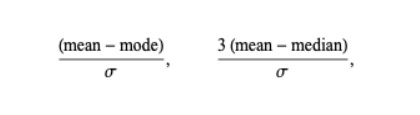
\includegraphics[width=9cm]{doc/latex/text/images/pearson-sk.jpg}
    \caption{Fórmulas para o 1º (esq.) e 2º (dir.) coeficientes de Pearson}
    \label{fig:pearson-sk}
\end{figure}


Quando uma distribuição é simétrica, ou seja, não possui valores em excesso tendendo acima ou abaixo da média, os coeficientes tendem a zero. Como exemplifica \citedirt{pearson1895}, há diversos fatores que podem influenciar na tendência de uma determinada variável:

\begin{citacao}
 Em primeiro lugar, o material medido pode ser heterogêneo e constituir de uma mistura de 2 ou mais materiais homogêneos. (...) A segunda classe de curvas de frequência ocorre no caso de material homogêneo quando a tendência de desvio para um lado de média é desigual a tendência para o outro lado. Curvas desse tipo aparecem em vários estudos físicos, econômicos e biológicos, por exemplo, em curvas de frequência para a altitude de um barômetro, em preços e taxas de juros de títulos mobiliários (...)
\end{citacao}

\section{Métodos de codificação}
Métodos comuns para representação codificada de dados categóricos no contento de \textit{Machine Learning} serão descritos nessa seção.

\subsection{One-hot encoding}
Método de codificação no qual cada valor é representado em sua forma codificada por um vetor de números inteiros no qual uma das posições corresponde ao valor 1 e todas as outras ao valor 0. \citedirt{google20} exemplifica o uso desse método com uma aplicação prática:

\begin{citacao}
Suponhamos que um dado \textit{dataset} de botânica descreva 15.000 diferentes espécies, cada uma indicada por uma \textit{string} identificadora única. Como parte da engenharia de parâmetros, você provavelmente codificaria esses identificadores como vetores \textit{one-hot}, os quais teriam tamanho 15.000.
\end{citacao}

\subsection{Embedding}
Método de codificação utilizado como alternativa ao \textit{one-hot encoding}. \citedirt{google20} define \textit{embedding} como "uma característica categórica representada como um valor contínuo" e "a tradução de um vetor de alta dimensionalidade para um espaço de baixa dimensionalidade". O mesmo autor exemplifica a aplicação prática do método:

\begin{citacao}
Você poderia representar as palavras em uma frase da língua Inglesa de duas maneiras: - Como um vetor esparso de milhões de elementos (alta dimensionalidade) no qual todos são valores inteiros. (...) - Como vários vetores densos de centenas de posições nos quais cada posição corresponde a um valor de ponto flutuante entre 0 e 1. Isso é um \textit{embedding}.
\end{citacao}

\section{Trabalhos Relacionados} \label{trabs-rel}
\label{trab-relacionados} 
No contexto de e-commerce, há trabalhos acadêmicos descrevendo diferentes abordagens, tais como sistemas de filtragem colaborativa que predizem avaliações por meio de fatorização de matrizes \cite{he17}, representam relações cliente/item utilizando grafos bipartidos \cite{wang19} e consideram fatores como críticas do usuário a sugestões geradas \cite{burke02} , sazonalidade e intenção de compra \cite{hwangbo18}.

Em sistema baseados em conteúdo ou com abordagens híbridas, é comum a utilização de resenhas escritas por usuários sobre os produtos como base para geração de sugestões, seja focando apenas na informação textual em si \cite{shoja19} ou relacionando com outros dados sobre os produtos em questão, tais como imagens \cite{wu20}.

Ainda no contexto de sistemas híbridos, há uma variedade de abordagens utilizadas para correlacionar produtos e clientes, tais como análise conjunta de múltiplos datasets e integração com dados provenientes de redes sociais \cite{li16}, cadeias de Markov \cite{yang20}, uso de agentes inteligentes baseados em lógica fuzzy \cite{yager00}, sistemas multi-agente \cite{aciar07}, entre outras.

No presente trabalho, em vez de trabalhar com avaliações numéricas dadas pelos usuários, as recomendações serão produzidas tendo com base somente no volume de vendas de um produto dentro de um determinado segmento de clientes. Isso permite que recomendações sejam geradas mesmo em aplicações que não coletam avaliações de clientes, ou em ERPs que possuem cadastros de pedidos simples, contando apenas com informações básicas do cliente, produto e transação, mas sem informações sobre a satisfação do consumidor no contexto pós-venda.

\textcolor{blue}{Padoin: vai citando mais trabalhos e no final precisamos dizer o que o teu tem de diferente dos demais}
\newline
\textcolor{blue}{Gabriel: alterei essa seção para citar mais trabalhos voltado a e-commerce e no último parágrafo destaco a diferença do meu para os demais}

\section{Considerações do Capítulo} \label{consid1}
Nesse capítulo foram apresentados áreas de conhecimento, tecnologias, técnicas e trabalho acadêmicos que possuem relação com o tema abordado nesse trabalho. No próximo capitulo serão apresentados os materiais e métodos e serem utilizados.
